\noindent The reflection attenuator \cite{pin_diode_designer_handbook} uses a quadrature hybrid and provides a wideband response and impednace match at the input and output ports.

  \begin{figure}[ht]
    \centering
    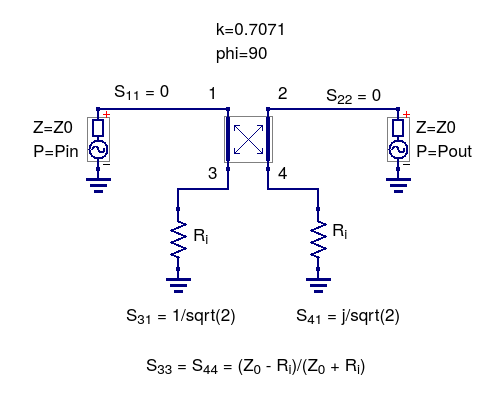
\includegraphics[width=10cm]{./images/reflection-attenuator-schematic.png}
    \caption{Reflection attenuator}
    \label{fig:reflection-attenuator-schematic}
  \end{figure}
  
\noindent The design equations can be obtained from S-parameter analysis.
  
  \begin{equation}
  S_{21} = S_{31} \cdot (-S_{33}) \cdot S_{23} + S_{41} \cdot (-S_{44}) \cdot S_{24} = \left( \frac{Z_0 - R_i}{Z_0 + R_i} \right) \cdot e^{j \cdot \pi/2}
  \end{equation}
  
\noindent Then, the attenuation (in dB) is given by:
  
  \begin{equation}
  	 \alpha = -20 \cdot log_{10} \left( \lvert S_{21} \rvert \right) = -20 \cdot log_{10} \left( \left| \frac{Z_0 - R_i}{Z_0 + R_i} \right| \right)
  	 \label{eq:attenuation-eq-reflection-attenuator}
  \end{equation}
  
\noindent Clearing $R_i$ from Eq. \ref{eq:attenuation-eq-reflection-attenuator}:
  
  \begin{equation}
  R_i = \begin{cases} Z_0 \cdot \frac{10^{-\alpha/20} - 1}{10^{-\alpha/20} + 1}, & \text{if  } R_i <  Z_0 \\ Z_0 \cdot \frac{1 + 10^{-\alpha/20}}{1 - 10^{-\alpha/20}}, & \text{if  } R_i > Z_0 \end{cases}
  \end{equation}
  
\noindent The power dissipation equations are derived similarly. Let be $P_{inc}$, $P_{refl}$, and $P_{diss}$ the incident, reflected and dissipated power in a resistor, respectively.
 
 \begin{equation}
 	P_{inc}^{R_i} = P_{in} \cdot \lvert S_{i1} \rvert^2
 \end{equation}
 
 \begin{equation}
 	P_{refl}^{R_i} = P_{in} \cdot \lvert S_{ii} \rvert^2
 \end{equation}
  
 \begin{equation}
 	P_{diss}^{R_i} = P_{inc}^{R_i} - P_{refl}^{R_i} = P_{in} \cdot \lvert S_{i1} \rvert^2 \cdot (1 - \lvert S_{ii} \rvert^2)
 \end{equation}
 
\noindent Being $S_{ii} = \frac{Z_0 - R_i}{Z_0 + R_i}$ and $S_{i1} = \lvert \frac{1}{\sqrt{2}}\rvert$
 
 \begin{equation}
 	  P_{diss}^{Ri} = \frac{P_{in}}{2} \cdot \left( 1  - \left| \frac{Z_0 - R_i}{Z_0 + R_i}\right|^2\right)
 \end{equation}
 
 \begin{equation}
  	P_{diss}^{Ri} = \frac{P_{in}}{2} \cdot \left( 1 - 10^{-\alpha/10}\right)
 \end{equation}
 
\noindent Thus, the power dissipated by the resistors is the same regardless $R_i < Z_0$ or $R_i > Z_0$
  
  \begin{figure}[ht]
    \centering
    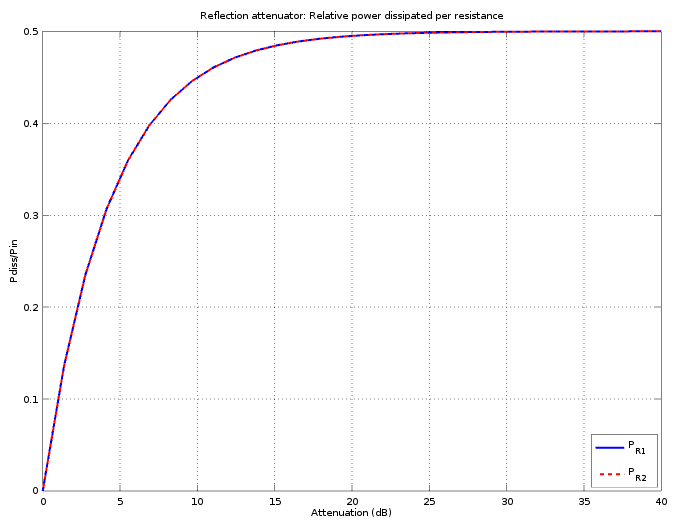
\includegraphics[width=10cm]{./images/reflective-att-relative-power-dissipation-50-Ohm.png}
    \caption{Power dissipated in the resistors in the reflective attenuator relative to the input power. $Z_{in} = Z_{out} = 50 \Omega$}
    \label{fig:reflective-att-relative-power-dissipation-50-Ohm}
  \end{figure}